% Graphic for TeX using PGF
% Title: C:\Users\Kaylen\CotWM\Doc\UML\AI_Combat.dia
% Creator: Dia v0.97.1
% CreationDate: Sat Mar 10 17:58:53 2012
% For: Kaylen
% \usepackage{tikz}
% The following commands are not supported in PSTricks at present
% We define them conditionally, so when they are implemented,
% this pgf file will use them.
\ifx\du\undefined
  \newlength{\du}
\fi
\setlength{\du}{15\unitlength}
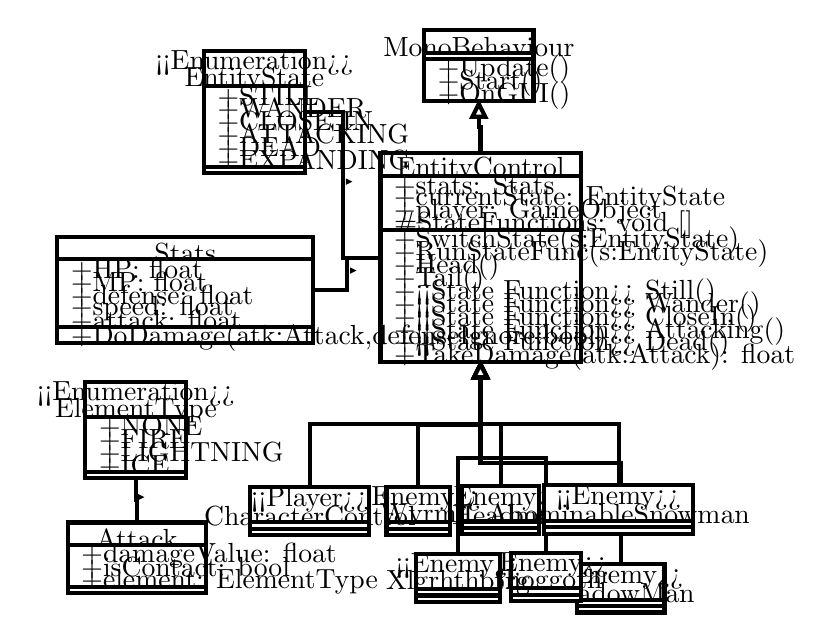
\begin{tikzpicture}
\pgftransformxscale{0.387817}
\pgftransformyscale{-0.387817}
\definecolor{dialinecolor}{rgb}{0.000000, 0.000000, 0.000000}
\pgfsetstrokecolor{dialinecolor}
\definecolor{dialinecolor}{rgb}{1.000000, 1.000000, 1.000000}
\pgfsetfillcolor{dialinecolor}
\pgfsetlinewidth{0.100000\du}
\pgfsetdash{}{0pt}
\definecolor{dialinecolor}{rgb}{1.000000, 1.000000, 1.000000}
\pgfsetfillcolor{dialinecolor}
\fill (-6.800000\du,4.250000\du)--(-6.800000\du,5.650000\du)--(5.635000\du,5.650000\du)--(5.635000\du,4.250000\du)--cycle;
\definecolor{dialinecolor}{rgb}{0.000000, 0.000000, 0.000000}
\pgfsetstrokecolor{dialinecolor}
\draw (-6.800000\du,4.250000\du)--(-6.800000\du,5.650000\du)--(5.635000\du,5.650000\du)--(5.635000\du,4.250000\du)--cycle;
% setfont left to latex
\definecolor{dialinecolor}{rgb}{0.000000, 0.000000, 0.000000}
\pgfsetstrokecolor{dialinecolor}
\node at (-0.582500\du,5.250000\du){EntityControl};
\definecolor{dialinecolor}{rgb}{1.000000, 1.000000, 1.000000}
\pgfsetfillcolor{dialinecolor}
\fill (-6.800000\du,5.650000\du)--(-6.800000\du,9.050000\du)--(5.635000\du,9.050000\du)--(5.635000\du,5.650000\du)--cycle;
\definecolor{dialinecolor}{rgb}{0.000000, 0.000000, 0.000000}
\pgfsetstrokecolor{dialinecolor}
\draw (-6.800000\du,5.650000\du)--(-6.800000\du,9.050000\du)--(5.635000\du,9.050000\du)--(5.635000\du,5.650000\du)--cycle;
% setfont left to latex
\definecolor{dialinecolor}{rgb}{0.000000, 0.000000, 0.000000}
\pgfsetstrokecolor{dialinecolor}
\node[anchor=west] at (-6.650000\du,6.310000\du){+stats: Stats};
% setfont left to latex
\definecolor{dialinecolor}{rgb}{0.000000, 0.000000, 0.000000}
\pgfsetstrokecolor{dialinecolor}
\node[anchor=west] at (-6.650000\du,7.110000\du){+currentState: EntityState};
% setfont left to latex
\definecolor{dialinecolor}{rgb}{0.000000, 0.000000, 0.000000}
\pgfsetstrokecolor{dialinecolor}
\node[anchor=west] at (-6.650000\du,7.910000\du){+player: GameObject};
% setfont left to latex
\definecolor{dialinecolor}{rgb}{0.000000, 0.000000, 0.000000}
\pgfsetstrokecolor{dialinecolor}
\node[anchor=west] at (-6.650000\du,8.710000\du){\#StateFunctions: void \ensuremath{[}\ensuremath{]}};
\definecolor{dialinecolor}{rgb}{1.000000, 1.000000, 1.000000}
\pgfsetfillcolor{dialinecolor}
\fill (-6.800000\du,9.050000\du)--(-6.800000\du,17.250000\du)--(5.635000\du,17.250000\du)--(5.635000\du,9.050000\du)--cycle;
\definecolor{dialinecolor}{rgb}{0.000000, 0.000000, 0.000000}
\pgfsetstrokecolor{dialinecolor}
\draw (-6.800000\du,9.050000\du)--(-6.800000\du,17.250000\du)--(5.635000\du,17.250000\du)--(5.635000\du,9.050000\du)--cycle;
% setfont left to latex
\definecolor{dialinecolor}{rgb}{0.000000, 0.000000, 0.000000}
\pgfsetstrokecolor{dialinecolor}
\node[anchor=west] at (-6.650000\du,9.710000\du){+SwitchState(s:EntityState)};
% setfont left to latex
\definecolor{dialinecolor}{rgb}{0.000000, 0.000000, 0.000000}
\pgfsetstrokecolor{dialinecolor}
\node[anchor=west] at (-6.650000\du,10.510000\du){+RunStateFunc(s:EntityState)};
% setfont left to latex
\definecolor{dialinecolor}{rgb}{0.000000, 0.000000, 0.000000}
\pgfsetstrokecolor{dialinecolor}
\node[anchor=west] at (-6.650000\du,11.310000\du){+Head()};
% setfont left to latex
\definecolor{dialinecolor}{rgb}{0.000000, 0.000000, 0.000000}
\pgfsetstrokecolor{dialinecolor}
\node[anchor=west] at (-6.650000\du,12.110000\du){+Tail()};
% setfont left to latex
\definecolor{dialinecolor}{rgb}{0.000000, 0.000000, 0.000000}
\pgfsetstrokecolor{dialinecolor}
\node[anchor=west] at (-6.650000\du,12.910000\du){+<<State Function>> Still()};
% setfont left to latex
\definecolor{dialinecolor}{rgb}{0.000000, 0.000000, 0.000000}
\pgfsetstrokecolor{dialinecolor}
\node[anchor=west] at (-6.650000\du,13.710000\du){+<<State Function>> Wander()};
% setfont left to latex
\definecolor{dialinecolor}{rgb}{0.000000, 0.000000, 0.000000}
\pgfsetstrokecolor{dialinecolor}
\node[anchor=west] at (-6.650000\du,14.510000\du){+<<State Function>> CloseIn()};
% setfont left to latex
\definecolor{dialinecolor}{rgb}{0.000000, 0.000000, 0.000000}
\pgfsetstrokecolor{dialinecolor}
\node[anchor=west] at (-6.650000\du,15.310000\du){+<<State Function>> Attacking()};
% setfont left to latex
\definecolor{dialinecolor}{rgb}{0.000000, 0.000000, 0.000000}
\pgfsetstrokecolor{dialinecolor}
\node[anchor=west] at (-6.650000\du,16.110000\du){+<<State Function>> Dead()};
% setfont left to latex
\definecolor{dialinecolor}{rgb}{0.000000, 0.000000, 0.000000}
\pgfsetstrokecolor{dialinecolor}
\node[anchor=west] at (-6.650000\du,16.910000\du){+TakeDamage(atk:Attack): float};
\pgfsetlinewidth{0.100000\du}
\pgfsetdash{}{0pt}
\definecolor{dialinecolor}{rgb}{1.000000, 1.000000, 1.000000}
\pgfsetfillcolor{dialinecolor}
\fill (-4.084275\du,-3.371875\du)--(-4.084275\du,-1.971875\du)--(2.710725\du,-1.971875\du)--(2.710725\du,-3.371875\du)--cycle;
\definecolor{dialinecolor}{rgb}{0.000000, 0.000000, 0.000000}
\pgfsetstrokecolor{dialinecolor}
\draw (-4.084275\du,-3.371875\du)--(-4.084275\du,-1.971875\du)--(2.710725\du,-1.971875\du)--(2.710725\du,-3.371875\du)--cycle;
% setfont left to latex
\definecolor{dialinecolor}{rgb}{0.000000, 0.000000, 0.000000}
\pgfsetstrokecolor{dialinecolor}
\node at (-0.686775\du,-2.371875\du){MonoBehaviour};
\definecolor{dialinecolor}{rgb}{1.000000, 1.000000, 1.000000}
\pgfsetfillcolor{dialinecolor}
\fill (-4.084275\du,-1.971875\du)--(-4.084275\du,-1.571875\du)--(2.710725\du,-1.571875\du)--(2.710725\du,-1.971875\du)--cycle;
\definecolor{dialinecolor}{rgb}{0.000000, 0.000000, 0.000000}
\pgfsetstrokecolor{dialinecolor}
\draw (-4.084275\du,-1.971875\du)--(-4.084275\du,-1.571875\du)--(2.710725\du,-1.571875\du)--(2.710725\du,-1.971875\du)--cycle;
\definecolor{dialinecolor}{rgb}{1.000000, 1.000000, 1.000000}
\pgfsetfillcolor{dialinecolor}
\fill (-4.084275\du,-1.571875\du)--(-4.084275\du,1.028125\du)--(2.710725\du,1.028125\du)--(2.710725\du,-1.571875\du)--cycle;
\definecolor{dialinecolor}{rgb}{0.000000, 0.000000, 0.000000}
\pgfsetstrokecolor{dialinecolor}
\draw (-4.084275\du,-1.571875\du)--(-4.084275\du,1.028125\du)--(2.710725\du,1.028125\du)--(2.710725\du,-1.571875\du)--cycle;
% setfont left to latex
\definecolor{dialinecolor}{rgb}{0.000000, 0.000000, 0.000000}
\pgfsetstrokecolor{dialinecolor}
\node[anchor=west] at (-3.934275\du,-0.911875\du){+Update()};
% setfont left to latex
\definecolor{dialinecolor}{rgb}{0.000000, 0.000000, 0.000000}
\pgfsetstrokecolor{dialinecolor}
\node[anchor=west] at (-3.934275\du,-0.111875\du){+Start()};
% setfont left to latex
\definecolor{dialinecolor}{rgb}{0.000000, 0.000000, 0.000000}
\pgfsetstrokecolor{dialinecolor}
\node[anchor=west] at (-3.934275\du,0.688125\du){+OnGUI()};
\pgfsetlinewidth{0.100000\du}
\pgfsetdash{}{0pt}
\pgfsetmiterjoin
\pgfsetbuttcap
{
\definecolor{dialinecolor}{rgb}{0.000000, 0.000000, 0.000000}
\pgfsetfillcolor{dialinecolor}
% was here!!!
\definecolor{dialinecolor}{rgb}{0.000000, 0.000000, 0.000000}
\pgfsetstrokecolor{dialinecolor}
\draw (-0.686775\du,1.078400\du)--(-0.686775\du,2.639000\du)--(-0.582500\du,2.639000\du)--(-0.582500\du,4.199600\du);
}
\definecolor{dialinecolor}{rgb}{0.000000, 0.000000, 0.000000}
\pgfsetstrokecolor{dialinecolor}
\draw (-0.686775\du,1.990203\du)--(-0.686775\du,2.639000\du)--(-0.582500\du,2.639000\du)--(-0.582500\du,4.199600\du);
\pgfsetmiterjoin
\definecolor{dialinecolor}{rgb}{1.000000, 1.000000, 1.000000}
\pgfsetfillcolor{dialinecolor}
\fill (-0.286775\du,1.990203\du)--(-0.686775\du,1.190203\du)--(-1.086775\du,1.990203\du)--cycle;
\pgfsetlinewidth{0.100000\du}
\pgfsetdash{}{0pt}
\pgfsetmiterjoin
\definecolor{dialinecolor}{rgb}{0.000000, 0.000000, 0.000000}
\pgfsetstrokecolor{dialinecolor}
\draw (-0.286775\du,1.990203\du)--(-0.686775\du,1.190203\du)--(-1.086775\du,1.990203\du)--cycle;
% setfont left to latex
\pgfsetlinewidth{0.100000\du}
\pgfsetdash{}{0pt}
\definecolor{dialinecolor}{rgb}{1.000000, 1.000000, 1.000000}
\pgfsetfillcolor{dialinecolor}
\fill (-17.771775\du,-2.109375\du)--(-17.771775\du,0.090625\du)--(-11.496775\du,0.090625\du)--(-11.496775\du,-2.109375\du)--cycle;
\definecolor{dialinecolor}{rgb}{0.000000, 0.000000, 0.000000}
\pgfsetstrokecolor{dialinecolor}
\draw (-17.771775\du,-2.109375\du)--(-17.771775\du,0.090625\du)--(-11.496775\du,0.090625\du)--(-11.496775\du,-2.109375\du)--cycle;
% setfont left to latex
\definecolor{dialinecolor}{rgb}{0.000000, 0.000000, 0.000000}
\pgfsetstrokecolor{dialinecolor}
\node at (-14.634275\du,-1.349375\du){<<Enumeration>>};
% setfont left to latex
\definecolor{dialinecolor}{rgb}{0.000000, 0.000000, 0.000000}
\pgfsetstrokecolor{dialinecolor}
\node at (-14.634275\du,-0.309375\du){EntityState};
\definecolor{dialinecolor}{rgb}{1.000000, 1.000000, 1.000000}
\pgfsetfillcolor{dialinecolor}
\fill (-17.771775\du,0.090625\du)--(-17.771775\du,5.090625\du)--(-11.496775\du,5.090625\du)--(-11.496775\du,0.090625\du)--cycle;
\definecolor{dialinecolor}{rgb}{0.000000, 0.000000, 0.000000}
\pgfsetstrokecolor{dialinecolor}
\draw (-17.771775\du,0.090625\du)--(-17.771775\du,5.090625\du)--(-11.496775\du,5.090625\du)--(-11.496775\du,0.090625\du)--cycle;
% setfont left to latex
\definecolor{dialinecolor}{rgb}{0.000000, 0.000000, 0.000000}
\pgfsetstrokecolor{dialinecolor}
\node[anchor=west] at (-17.621775\du,0.750625\du){+STILL};
% setfont left to latex
\definecolor{dialinecolor}{rgb}{0.000000, 0.000000, 0.000000}
\pgfsetstrokecolor{dialinecolor}
\node[anchor=west] at (-17.621775\du,1.550625\du){+WANDER};
% setfont left to latex
\definecolor{dialinecolor}{rgb}{0.000000, 0.000000, 0.000000}
\pgfsetstrokecolor{dialinecolor}
\node[anchor=west] at (-17.621775\du,2.350625\du){+CLOSE\_IN};
% setfont left to latex
\definecolor{dialinecolor}{rgb}{0.000000, 0.000000, 0.000000}
\pgfsetstrokecolor{dialinecolor}
\node[anchor=west] at (-17.621775\du,3.150625\du){+ATTACKING};
% setfont left to latex
\definecolor{dialinecolor}{rgb}{0.000000, 0.000000, 0.000000}
\pgfsetstrokecolor{dialinecolor}
\node[anchor=west] at (-17.621775\du,3.950625\du){+DEAD};
% setfont left to latex
\definecolor{dialinecolor}{rgb}{0.000000, 0.000000, 0.000000}
\pgfsetstrokecolor{dialinecolor}
\node[anchor=west] at (-17.621775\du,4.750625\du){+EXPANDING};
\definecolor{dialinecolor}{rgb}{1.000000, 1.000000, 1.000000}
\pgfsetfillcolor{dialinecolor}
\fill (-17.771775\du,5.090625\du)--(-17.771775\du,5.490625\du)--(-11.496775\du,5.490625\du)--(-11.496775\du,5.090625\du)--cycle;
\definecolor{dialinecolor}{rgb}{0.000000, 0.000000, 0.000000}
\pgfsetstrokecolor{dialinecolor}
\draw (-17.771775\du,5.090625\du)--(-17.771775\du,5.490625\du)--(-11.496775\du,5.490625\du)--(-11.496775\du,5.090625\du)--cycle;
\pgfsetlinewidth{0.100000\du}
\pgfsetdash{}{0pt}
\pgfsetmiterjoin
\pgfsetbuttcap
{
\definecolor{dialinecolor}{rgb}{0.000000, 0.000000, 0.000000}
\pgfsetfillcolor{dialinecolor}
% was here!!!
\definecolor{dialinecolor}{rgb}{0.000000, 0.000000, 0.000000}
\pgfsetstrokecolor{dialinecolor}
\draw (-11.446386\du,1.690625\du)--(-9.148384\du,1.690625\du)--(-9.148384\du,10.750000\du)--(-6.850383\du,10.750000\du);
}
% setfont left to latex
\definecolor{dialinecolor}{rgb}{0.000000, 0.000000, 0.000000}
\pgfsetfillcolor{dialinecolor}
\fill (-8.948384\du,6.220312\du)--(-8.948384\du,5.820312\du)--(-8.548384\du,6.020312\du)--cycle;
\pgfsetlinewidth{0.100000\du}
\pgfsetdash{}{0pt}
\definecolor{dialinecolor}{rgb}{1.000000, 1.000000, 1.000000}
\pgfsetfillcolor{dialinecolor}
\fill (-26.871775\du,9.440625\du)--(-26.871775\du,10.840625\du)--(-10.971775\du,10.840625\du)--(-10.971775\du,9.440625\du)--cycle;
\definecolor{dialinecolor}{rgb}{0.000000, 0.000000, 0.000000}
\pgfsetstrokecolor{dialinecolor}
\draw (-26.871775\du,9.440625\du)--(-26.871775\du,10.840625\du)--(-10.971775\du,10.840625\du)--(-10.971775\du,9.440625\du)--cycle;
% setfont left to latex
\definecolor{dialinecolor}{rgb}{0.000000, 0.000000, 0.000000}
\pgfsetstrokecolor{dialinecolor}
\node at (-18.921775\du,10.440625\du){Stats};
\definecolor{dialinecolor}{rgb}{1.000000, 1.000000, 1.000000}
\pgfsetfillcolor{dialinecolor}
\fill (-26.871775\du,10.840625\du)--(-26.871775\du,15.040625\du)--(-10.971775\du,15.040625\du)--(-10.971775\du,10.840625\du)--cycle;
\definecolor{dialinecolor}{rgb}{0.000000, 0.000000, 0.000000}
\pgfsetstrokecolor{dialinecolor}
\draw (-26.871775\du,10.840625\du)--(-26.871775\du,15.040625\du)--(-10.971775\du,15.040625\du)--(-10.971775\du,10.840625\du)--cycle;
% setfont left to latex
\definecolor{dialinecolor}{rgb}{0.000000, 0.000000, 0.000000}
\pgfsetstrokecolor{dialinecolor}
\node[anchor=west] at (-26.721775\du,11.500625\du){+HP: float};
% setfont left to latex
\definecolor{dialinecolor}{rgb}{0.000000, 0.000000, 0.000000}
\pgfsetstrokecolor{dialinecolor}
\node[anchor=west] at (-26.721775\du,12.300625\du){+MP: float};
% setfont left to latex
\definecolor{dialinecolor}{rgb}{0.000000, 0.000000, 0.000000}
\pgfsetstrokecolor{dialinecolor}
\node[anchor=west] at (-26.721775\du,13.100625\du){+defense: float};
% setfont left to latex
\definecolor{dialinecolor}{rgb}{0.000000, 0.000000, 0.000000}
\pgfsetstrokecolor{dialinecolor}
\node[anchor=west] at (-26.721775\du,13.900625\du){+speed: float};
% setfont left to latex
\definecolor{dialinecolor}{rgb}{0.000000, 0.000000, 0.000000}
\pgfsetstrokecolor{dialinecolor}
\node[anchor=west] at (-26.721775\du,14.700625\du){+attack: float};
\definecolor{dialinecolor}{rgb}{1.000000, 1.000000, 1.000000}
\pgfsetfillcolor{dialinecolor}
\fill (-26.871775\du,15.040625\du)--(-26.871775\du,16.040625\du)--(-10.971775\du,16.040625\du)--(-10.971775\du,15.040625\du)--cycle;
\definecolor{dialinecolor}{rgb}{0.000000, 0.000000, 0.000000}
\pgfsetstrokecolor{dialinecolor}
\draw (-26.871775\du,15.040625\du)--(-26.871775\du,16.040625\du)--(-10.971775\du,16.040625\du)--(-10.971775\du,15.040625\du)--cycle;
% setfont left to latex
\definecolor{dialinecolor}{rgb}{0.000000, 0.000000, 0.000000}
\pgfsetstrokecolor{dialinecolor}
\node[anchor=west] at (-26.721775\du,15.700625\du){+DoDamage(atk:Attack,defenseIgnore:bool)};
\pgfsetlinewidth{0.100000\du}
\pgfsetdash{}{0pt}
\definecolor{dialinecolor}{rgb}{1.000000, 1.000000, 1.000000}
\pgfsetfillcolor{dialinecolor}
\fill (-26.221775\du,27.190625\du)--(-26.221775\du,28.590625\du)--(-17.636775\du,28.590625\du)--(-17.636775\du,27.190625\du)--cycle;
\definecolor{dialinecolor}{rgb}{0.000000, 0.000000, 0.000000}
\pgfsetstrokecolor{dialinecolor}
\draw (-26.221775\du,27.190625\du)--(-26.221775\du,28.590625\du)--(-17.636775\du,28.590625\du)--(-17.636775\du,27.190625\du)--cycle;
% setfont left to latex
\definecolor{dialinecolor}{rgb}{0.000000, 0.000000, 0.000000}
\pgfsetstrokecolor{dialinecolor}
\node at (-21.929275\du,28.190625\du){Attack};
\definecolor{dialinecolor}{rgb}{1.000000, 1.000000, 1.000000}
\pgfsetfillcolor{dialinecolor}
\fill (-26.221775\du,28.590625\du)--(-26.221775\du,31.190625\du)--(-17.636775\du,31.190625\du)--(-17.636775\du,28.590625\du)--cycle;
\definecolor{dialinecolor}{rgb}{0.000000, 0.000000, 0.000000}
\pgfsetstrokecolor{dialinecolor}
\draw (-26.221775\du,28.590625\du)--(-26.221775\du,31.190625\du)--(-17.636775\du,31.190625\du)--(-17.636775\du,28.590625\du)--cycle;
% setfont left to latex
\definecolor{dialinecolor}{rgb}{0.000000, 0.000000, 0.000000}
\pgfsetstrokecolor{dialinecolor}
\node[anchor=west] at (-26.071775\du,29.250625\du){+damageValue: float};
% setfont left to latex
\definecolor{dialinecolor}{rgb}{0.000000, 0.000000, 0.000000}
\pgfsetstrokecolor{dialinecolor}
\node[anchor=west] at (-26.071775\du,30.050625\du){+isContact: bool};
% setfont left to latex
\definecolor{dialinecolor}{rgb}{0.000000, 0.000000, 0.000000}
\pgfsetstrokecolor{dialinecolor}
\node[anchor=west] at (-26.071775\du,30.850625\du){+element: ElementType};
\definecolor{dialinecolor}{rgb}{1.000000, 1.000000, 1.000000}
\pgfsetfillcolor{dialinecolor}
\fill (-26.221775\du,31.190625\du)--(-26.221775\du,31.590625\du)--(-17.636775\du,31.590625\du)--(-17.636775\du,31.190625\du)--cycle;
\definecolor{dialinecolor}{rgb}{0.000000, 0.000000, 0.000000}
\pgfsetstrokecolor{dialinecolor}
\draw (-26.221775\du,31.190625\du)--(-26.221775\du,31.590625\du)--(-17.636775\du,31.590625\du)--(-17.636775\du,31.190625\du)--cycle;
\pgfsetlinewidth{0.100000\du}
\pgfsetdash{}{0pt}
\definecolor{dialinecolor}{rgb}{1.000000, 1.000000, 1.000000}
\pgfsetfillcolor{dialinecolor}
\fill (-25.126775\du,18.445625\du)--(-25.126775\du,20.645625\du)--(-18.851775\du,20.645625\du)--(-18.851775\du,18.445625\du)--cycle;
\definecolor{dialinecolor}{rgb}{0.000000, 0.000000, 0.000000}
\pgfsetstrokecolor{dialinecolor}
\draw (-25.126775\du,18.445625\du)--(-25.126775\du,20.645625\du)--(-18.851775\du,20.645625\du)--(-18.851775\du,18.445625\du)--cycle;
% setfont left to latex
\definecolor{dialinecolor}{rgb}{0.000000, 0.000000, 0.000000}
\pgfsetstrokecolor{dialinecolor}
\node at (-21.989275\du,19.205625\du){<<Enumeration>>};
% setfont left to latex
\definecolor{dialinecolor}{rgb}{0.000000, 0.000000, 0.000000}
\pgfsetstrokecolor{dialinecolor}
\node at (-21.989275\du,20.245625\du){ElementType};
\definecolor{dialinecolor}{rgb}{1.000000, 1.000000, 1.000000}
\pgfsetfillcolor{dialinecolor}
\fill (-25.126775\du,20.645625\du)--(-25.126775\du,24.045625\du)--(-18.851775\du,24.045625\du)--(-18.851775\du,20.645625\du)--cycle;
\definecolor{dialinecolor}{rgb}{0.000000, 0.000000, 0.000000}
\pgfsetstrokecolor{dialinecolor}
\draw (-25.126775\du,20.645625\du)--(-25.126775\du,24.045625\du)--(-18.851775\du,24.045625\du)--(-18.851775\du,20.645625\du)--cycle;
% setfont left to latex
\definecolor{dialinecolor}{rgb}{0.000000, 0.000000, 0.000000}
\pgfsetstrokecolor{dialinecolor}
\node[anchor=west] at (-24.976775\du,21.305625\du){+NONE};
% setfont left to latex
\definecolor{dialinecolor}{rgb}{0.000000, 0.000000, 0.000000}
\pgfsetstrokecolor{dialinecolor}
\node[anchor=west] at (-24.976775\du,22.105625\du){+FIRE};
% setfont left to latex
\definecolor{dialinecolor}{rgb}{0.000000, 0.000000, 0.000000}
\pgfsetstrokecolor{dialinecolor}
\node[anchor=west] at (-24.976775\du,22.905625\du){+LIGHTNING};
% setfont left to latex
\definecolor{dialinecolor}{rgb}{0.000000, 0.000000, 0.000000}
\pgfsetstrokecolor{dialinecolor}
\node[anchor=west] at (-24.976775\du,23.705625\du){+ICE};
\definecolor{dialinecolor}{rgb}{1.000000, 1.000000, 1.000000}
\pgfsetfillcolor{dialinecolor}
\fill (-25.126775\du,24.045625\du)--(-25.126775\du,24.445625\du)--(-18.851775\du,24.445625\du)--(-18.851775\du,24.045625\du)--cycle;
\definecolor{dialinecolor}{rgb}{0.000000, 0.000000, 0.000000}
\pgfsetstrokecolor{dialinecolor}
\draw (-25.126775\du,24.045625\du)--(-25.126775\du,24.445625\du)--(-18.851775\du,24.445625\du)--(-18.851775\du,24.045625\du)--cycle;
\pgfsetlinewidth{0.100000\du}
\pgfsetdash{}{0pt}
\pgfsetmiterjoin
\pgfsetbuttcap
{
\definecolor{dialinecolor}{rgb}{0.000000, 0.000000, 0.000000}
\pgfsetfillcolor{dialinecolor}
% was here!!!
\definecolor{dialinecolor}{rgb}{0.000000, 0.000000, 0.000000}
\pgfsetstrokecolor{dialinecolor}
\draw (-21.929275\du,27.140350\du)--(-21.929275\du,25.818174\du)--(-21.989275\du,25.818174\du)--(-21.989275\du,24.495997\du);
}
% setfont left to latex
\definecolor{dialinecolor}{rgb}{0.000000, 0.000000, 0.000000}
\pgfsetfillcolor{dialinecolor}
\fill (-21.859275\du,25.818174\du)--(-21.859275\du,25.418174\du)--(-21.459275\du,25.618174\du)--cycle;
\pgfsetlinewidth{0.100000\du}
\pgfsetdash{}{0pt}
\pgfsetmiterjoin
\pgfsetbuttcap
{
\definecolor{dialinecolor}{rgb}{0.000000, 0.000000, 0.000000}
\pgfsetfillcolor{dialinecolor}
% was here!!!
\definecolor{dialinecolor}{rgb}{0.000000, 0.000000, 0.000000}
\pgfsetstrokecolor{dialinecolor}
\draw (-6.850383\du,10.750000\du)--(-8.885835\du,10.750000\du)--(-8.885835\du,12.740625\du)--(-10.921287\du,12.740625\du);
}
% setfont left to latex
\definecolor{dialinecolor}{rgb}{0.000000, 0.000000, 0.000000}
\pgfsetfillcolor{dialinecolor}
\fill (-8.685835\du,11.745312\du)--(-8.685835\du,11.345312\du)--(-8.285835\du,11.545312\du)--cycle;
\pgfsetlinewidth{0.100000\du}
\pgfsetdash{}{0pt}
\definecolor{dialinecolor}{rgb}{1.000000, 1.000000, 1.000000}
\pgfsetfillcolor{dialinecolor}
\fill (-1.726775\du,24.933125\du)--(-1.726775\du,27.133125\du)--(3.063225\du,27.133125\du)--(3.063225\du,24.933125\du)--cycle;
\definecolor{dialinecolor}{rgb}{0.000000, 0.000000, 0.000000}
\pgfsetstrokecolor{dialinecolor}
\draw (-1.726775\du,24.933125\du)--(-1.726775\du,27.133125\du)--(3.063225\du,27.133125\du)--(3.063225\du,24.933125\du)--cycle;
% setfont left to latex
\definecolor{dialinecolor}{rgb}{0.000000, 0.000000, 0.000000}
\pgfsetstrokecolor{dialinecolor}
\node at (0.668225\du,25.693125\du){<<Enemy>>};
% setfont left to latex
\definecolor{dialinecolor}{rgb}{0.000000, 0.000000, 0.000000}
\pgfsetstrokecolor{dialinecolor}
\node at (0.668225\du,26.733125\du){FHeadman};
\definecolor{dialinecolor}{rgb}{1.000000, 1.000000, 1.000000}
\pgfsetfillcolor{dialinecolor}
\fill (-1.726775\du,27.133125\du)--(-1.726775\du,27.533125\du)--(3.063225\du,27.533125\du)--(3.063225\du,27.133125\du)--cycle;
\definecolor{dialinecolor}{rgb}{0.000000, 0.000000, 0.000000}
\pgfsetstrokecolor{dialinecolor}
\draw (-1.726775\du,27.133125\du)--(-1.726775\du,27.533125\du)--(3.063225\du,27.533125\du)--(3.063225\du,27.133125\du)--cycle;
\definecolor{dialinecolor}{rgb}{1.000000, 1.000000, 1.000000}
\pgfsetfillcolor{dialinecolor}
\fill (-1.726775\du,27.533125\du)--(-1.726775\du,27.933125\du)--(3.063225\du,27.933125\du)--(3.063225\du,27.533125\du)--cycle;
\definecolor{dialinecolor}{rgb}{0.000000, 0.000000, 0.000000}
\pgfsetstrokecolor{dialinecolor}
\draw (-1.726775\du,27.533125\du)--(-1.726775\du,27.933125\du)--(3.063225\du,27.933125\du)--(3.063225\du,27.533125\du)--cycle;
\pgfsetlinewidth{0.100000\du}
\pgfsetdash{}{0pt}
\pgfsetmiterjoin
\pgfsetbuttcap
{
\definecolor{dialinecolor}{rgb}{0.000000, 0.000000, 0.000000}
\pgfsetfillcolor{dialinecolor}
% was here!!!
\definecolor{dialinecolor}{rgb}{0.000000, 0.000000, 0.000000}
\pgfsetstrokecolor{dialinecolor}
\draw (-0.582500\du,17.300400\du)--(-0.582500\du,21.091573\du)--(0.668225\du,21.091573\du)--(0.668225\du,24.882747\du);
}
\definecolor{dialinecolor}{rgb}{0.000000, 0.000000, 0.000000}
\pgfsetstrokecolor{dialinecolor}
\draw (-0.582500\du,18.212203\du)--(-0.582500\du,21.091573\du)--(0.668225\du,21.091573\du)--(0.668225\du,24.882747\du);
\pgfsetmiterjoin
\definecolor{dialinecolor}{rgb}{1.000000, 1.000000, 1.000000}
\pgfsetfillcolor{dialinecolor}
\fill (-0.182500\du,18.212203\du)--(-0.582500\du,17.412203\du)--(-0.982500\du,18.212203\du)--cycle;
\pgfsetlinewidth{0.100000\du}
\pgfsetdash{}{0pt}
\pgfsetmiterjoin
\definecolor{dialinecolor}{rgb}{0.000000, 0.000000, 0.000000}
\pgfsetstrokecolor{dialinecolor}
\draw (-0.182500\du,18.212203\du)--(-0.582500\du,17.412203\du)--(-0.982500\du,18.212203\du)--cycle;
% setfont left to latex
\pgfsetlinewidth{0.100000\du}
\pgfsetdash{}{0pt}
\definecolor{dialinecolor}{rgb}{1.000000, 1.000000, 1.000000}
\pgfsetfillcolor{dialinecolor}
\fill (5.423225\du,29.783125\du)--(5.423225\du,31.983125\du)--(10.840725\du,31.983125\du)--(10.840725\du,29.783125\du)--cycle;
\definecolor{dialinecolor}{rgb}{0.000000, 0.000000, 0.000000}
\pgfsetstrokecolor{dialinecolor}
\draw (5.423225\du,29.783125\du)--(5.423225\du,31.983125\du)--(10.840725\du,31.983125\du)--(10.840725\du,29.783125\du)--cycle;
% setfont left to latex
\definecolor{dialinecolor}{rgb}{0.000000, 0.000000, 0.000000}
\pgfsetstrokecolor{dialinecolor}
\node at (8.131975\du,30.543125\du){<<Enemy>>};
% setfont left to latex
\definecolor{dialinecolor}{rgb}{0.000000, 0.000000, 0.000000}
\pgfsetstrokecolor{dialinecolor}
\node at (8.131975\du,31.583125\du){ShadowMan};
\definecolor{dialinecolor}{rgb}{1.000000, 1.000000, 1.000000}
\pgfsetfillcolor{dialinecolor}
\fill (5.423225\du,31.983125\du)--(5.423225\du,32.383125\du)--(10.840725\du,32.383125\du)--(10.840725\du,31.983125\du)--cycle;
\definecolor{dialinecolor}{rgb}{0.000000, 0.000000, 0.000000}
\pgfsetstrokecolor{dialinecolor}
\draw (5.423225\du,31.983125\du)--(5.423225\du,32.383125\du)--(10.840725\du,32.383125\du)--(10.840725\du,31.983125\du)--cycle;
\definecolor{dialinecolor}{rgb}{1.000000, 1.000000, 1.000000}
\pgfsetfillcolor{dialinecolor}
\fill (5.423225\du,32.383125\du)--(5.423225\du,32.783125\du)--(10.840725\du,32.783125\du)--(10.840725\du,32.383125\du)--cycle;
\definecolor{dialinecolor}{rgb}{0.000000, 0.000000, 0.000000}
\pgfsetstrokecolor{dialinecolor}
\draw (5.423225\du,32.383125\du)--(5.423225\du,32.783125\du)--(10.840725\du,32.783125\du)--(10.840725\du,32.383125\du)--cycle;
\pgfsetlinewidth{0.100000\du}
\pgfsetdash{}{0pt}
\definecolor{dialinecolor}{rgb}{1.000000, 1.000000, 1.000000}
\pgfsetfillcolor{dialinecolor}
\fill (1.323225\du,29.083125\du)--(1.323225\du,31.283125\du)--(5.683225\du,31.283125\du)--(5.683225\du,29.083125\du)--cycle;
\definecolor{dialinecolor}{rgb}{0.000000, 0.000000, 0.000000}
\pgfsetstrokecolor{dialinecolor}
\draw (1.323225\du,29.083125\du)--(1.323225\du,31.283125\du)--(5.683225\du,31.283125\du)--(5.683225\du,29.083125\du)--cycle;
% setfont left to latex
\definecolor{dialinecolor}{rgb}{0.000000, 0.000000, 0.000000}
\pgfsetstrokecolor{dialinecolor}
\node at (3.503225\du,29.843125\du){<<Enemy>>};
% setfont left to latex
\definecolor{dialinecolor}{rgb}{0.000000, 0.000000, 0.000000}
\pgfsetstrokecolor{dialinecolor}
\node at (3.503225\du,30.883125\du){Shoggoth};
\definecolor{dialinecolor}{rgb}{1.000000, 1.000000, 1.000000}
\pgfsetfillcolor{dialinecolor}
\fill (1.323225\du,31.283125\du)--(1.323225\du,31.683125\du)--(5.683225\du,31.683125\du)--(5.683225\du,31.283125\du)--cycle;
\definecolor{dialinecolor}{rgb}{0.000000, 0.000000, 0.000000}
\pgfsetstrokecolor{dialinecolor}
\draw (1.323225\du,31.283125\du)--(1.323225\du,31.683125\du)--(5.683225\du,31.683125\du)--(5.683225\du,31.283125\du)--cycle;
\definecolor{dialinecolor}{rgb}{1.000000, 1.000000, 1.000000}
\pgfsetfillcolor{dialinecolor}
\fill (1.323225\du,31.683125\du)--(1.323225\du,32.083125\du)--(5.683225\du,32.083125\du)--(5.683225\du,31.683125\du)--cycle;
\definecolor{dialinecolor}{rgb}{0.000000, 0.000000, 0.000000}
\pgfsetstrokecolor{dialinecolor}
\draw (1.323225\du,31.683125\du)--(1.323225\du,32.083125\du)--(5.683225\du,32.083125\du)--(5.683225\du,31.683125\du)--cycle;
\pgfsetlinewidth{0.100000\du}
\pgfsetdash{}{0pt}
\definecolor{dialinecolor}{rgb}{1.000000, 1.000000, 1.000000}
\pgfsetfillcolor{dialinecolor}
\fill (-6.426775\du,24.983125\du)--(-6.426775\du,27.183125\du)--(-2.461775\du,27.183125\du)--(-2.461775\du,24.983125\du)--cycle;
\definecolor{dialinecolor}{rgb}{0.000000, 0.000000, 0.000000}
\pgfsetstrokecolor{dialinecolor}
\draw (-6.426775\du,24.983125\du)--(-6.426775\du,27.183125\du)--(-2.461775\du,27.183125\du)--(-2.461775\du,24.983125\du)--cycle;
% setfont left to latex
\definecolor{dialinecolor}{rgb}{0.000000, 0.000000, 0.000000}
\pgfsetstrokecolor{dialinecolor}
\node at (-4.444275\du,25.743125\du){<<Enemy>>};
% setfont left to latex
\definecolor{dialinecolor}{rgb}{0.000000, 0.000000, 0.000000}
\pgfsetstrokecolor{dialinecolor}
\node at (-4.444275\du,26.783125\du){Wyrm};
\definecolor{dialinecolor}{rgb}{1.000000, 1.000000, 1.000000}
\pgfsetfillcolor{dialinecolor}
\fill (-6.426775\du,27.183125\du)--(-6.426775\du,27.583125\du)--(-2.461775\du,27.583125\du)--(-2.461775\du,27.183125\du)--cycle;
\definecolor{dialinecolor}{rgb}{0.000000, 0.000000, 0.000000}
\pgfsetstrokecolor{dialinecolor}
\draw (-6.426775\du,27.183125\du)--(-6.426775\du,27.583125\du)--(-2.461775\du,27.583125\du)--(-2.461775\du,27.183125\du)--cycle;
\definecolor{dialinecolor}{rgb}{1.000000, 1.000000, 1.000000}
\pgfsetfillcolor{dialinecolor}
\fill (-6.426775\du,27.583125\du)--(-6.426775\du,27.983125\du)--(-2.461775\du,27.983125\du)--(-2.461775\du,27.583125\du)--cycle;
\definecolor{dialinecolor}{rgb}{0.000000, 0.000000, 0.000000}
\pgfsetstrokecolor{dialinecolor}
\draw (-6.426775\du,27.583125\du)--(-6.426775\du,27.983125\du)--(-2.461775\du,27.983125\du)--(-2.461775\du,27.583125\du)--cycle;
\pgfsetlinewidth{0.100000\du}
\pgfsetdash{}{0pt}
\pgfsetmiterjoin
\pgfsetbuttcap
{
\definecolor{dialinecolor}{rgb}{0.000000, 0.000000, 0.000000}
\pgfsetfillcolor{dialinecolor}
% was here!!!
\definecolor{dialinecolor}{rgb}{0.000000, 0.000000, 0.000000}
\pgfsetstrokecolor{dialinecolor}
\draw (-0.582500\du,17.300400\du)--(-0.582500\du,21.116573\du)--(-4.444275\du,21.116573\du)--(-4.444275\du,24.932747\du);
}
\definecolor{dialinecolor}{rgb}{0.000000, 0.000000, 0.000000}
\pgfsetstrokecolor{dialinecolor}
\draw (-0.582500\du,18.212203\du)--(-0.582500\du,21.116573\du)--(-4.444275\du,21.116573\du)--(-4.444275\du,24.932747\du);
\pgfsetmiterjoin
\definecolor{dialinecolor}{rgb}{1.000000, 1.000000, 1.000000}
\pgfsetfillcolor{dialinecolor}
\fill (-0.182500\du,18.212203\du)--(-0.582500\du,17.412203\du)--(-0.982500\du,18.212203\du)--cycle;
\pgfsetlinewidth{0.100000\du}
\pgfsetdash{}{0pt}
\pgfsetmiterjoin
\definecolor{dialinecolor}{rgb}{0.000000, 0.000000, 0.000000}
\pgfsetstrokecolor{dialinecolor}
\draw (-0.182500\du,18.212203\du)--(-0.582500\du,17.412203\du)--(-0.982500\du,18.212203\du)--cycle;
% setfont left to latex
\pgfsetlinewidth{0.100000\du}
\pgfsetdash{}{0pt}
\pgfsetmiterjoin
\pgfsetbuttcap
{
\definecolor{dialinecolor}{rgb}{0.000000, 0.000000, 0.000000}
\pgfsetfillcolor{dialinecolor}
% was here!!!
\definecolor{dialinecolor}{rgb}{0.000000, 0.000000, 0.000000}
\pgfsetstrokecolor{dialinecolor}
\draw (-0.582500\du,17.250000\du)--(-0.582500\du,23.491373\du)--(8.131975\du,23.491373\du)--(8.131975\du,29.732747\du);
}
\definecolor{dialinecolor}{rgb}{0.000000, 0.000000, 0.000000}
\pgfsetstrokecolor{dialinecolor}
\draw (-0.582500\du,18.161803\du)--(-0.582500\du,23.491373\du)--(8.131975\du,23.491373\du)--(8.131975\du,29.732747\du);
\pgfsetmiterjoin
\definecolor{dialinecolor}{rgb}{1.000000, 1.000000, 1.000000}
\pgfsetfillcolor{dialinecolor}
\fill (-0.182500\du,18.161803\du)--(-0.582500\du,17.361803\du)--(-0.982500\du,18.161803\du)--cycle;
\pgfsetlinewidth{0.100000\du}
\pgfsetdash{}{0pt}
\pgfsetmiterjoin
\definecolor{dialinecolor}{rgb}{0.000000, 0.000000, 0.000000}
\pgfsetstrokecolor{dialinecolor}
\draw (-0.182500\du,18.161803\du)--(-0.582500\du,17.361803\du)--(-0.982500\du,18.161803\du)--cycle;
% setfont left to latex
\pgfsetlinewidth{0.100000\du}
\pgfsetdash{}{0pt}
\pgfsetmiterjoin
\pgfsetbuttcap
{
\definecolor{dialinecolor}{rgb}{0.000000, 0.000000, 0.000000}
\pgfsetfillcolor{dialinecolor}
% was here!!!
\definecolor{dialinecolor}{rgb}{0.000000, 0.000000, 0.000000}
\pgfsetstrokecolor{dialinecolor}
\draw (-0.582500\du,17.300400\du)--(-0.582500\du,23.166573\du)--(3.503225\du,23.166573\du)--(3.503225\du,29.032747\du);
}
\definecolor{dialinecolor}{rgb}{0.000000, 0.000000, 0.000000}
\pgfsetstrokecolor{dialinecolor}
\draw (-0.582500\du,18.212203\du)--(-0.582500\du,23.166573\du)--(3.503225\du,23.166573\du)--(3.503225\du,29.032747\du);
\pgfsetmiterjoin
\definecolor{dialinecolor}{rgb}{1.000000, 1.000000, 1.000000}
\pgfsetfillcolor{dialinecolor}
\fill (-0.182500\du,18.212203\du)--(-0.582500\du,17.412203\du)--(-0.982500\du,18.212203\du)--cycle;
\pgfsetlinewidth{0.100000\du}
\pgfsetdash{}{0pt}
\pgfsetmiterjoin
\definecolor{dialinecolor}{rgb}{0.000000, 0.000000, 0.000000}
\pgfsetstrokecolor{dialinecolor}
\draw (-0.182500\du,18.212203\du)--(-0.582500\du,17.412203\du)--(-0.982500\du,18.212203\du)--cycle;
% setfont left to latex
\pgfsetlinewidth{0.100000\du}
\pgfsetdash{}{0pt}
\definecolor{dialinecolor}{rgb}{1.000000, 1.000000, 1.000000}
\pgfsetfillcolor{dialinecolor}
\fill (3.373225\du,24.883125\du)--(3.373225\du,27.083125\du)--(12.623225\du,27.083125\du)--(12.623225\du,24.883125\du)--cycle;
\definecolor{dialinecolor}{rgb}{0.000000, 0.000000, 0.000000}
\pgfsetstrokecolor{dialinecolor}
\draw (3.373225\du,24.883125\du)--(3.373225\du,27.083125\du)--(12.623225\du,27.083125\du)--(12.623225\du,24.883125\du)--cycle;
% setfont left to latex
\definecolor{dialinecolor}{rgb}{0.000000, 0.000000, 0.000000}
\pgfsetstrokecolor{dialinecolor}
\node at (7.998225\du,25.643125\du){<<Enemy>>};
% setfont left to latex
\definecolor{dialinecolor}{rgb}{0.000000, 0.000000, 0.000000}
\pgfsetstrokecolor{dialinecolor}
\node at (7.998225\du,26.683125\du){AbominableSnowman};
\definecolor{dialinecolor}{rgb}{1.000000, 1.000000, 1.000000}
\pgfsetfillcolor{dialinecolor}
\fill (3.373225\du,27.083125\du)--(3.373225\du,27.483125\du)--(12.623225\du,27.483125\du)--(12.623225\du,27.083125\du)--cycle;
\definecolor{dialinecolor}{rgb}{0.000000, 0.000000, 0.000000}
\pgfsetstrokecolor{dialinecolor}
\draw (3.373225\du,27.083125\du)--(3.373225\du,27.483125\du)--(12.623225\du,27.483125\du)--(12.623225\du,27.083125\du)--cycle;
\definecolor{dialinecolor}{rgb}{1.000000, 1.000000, 1.000000}
\pgfsetfillcolor{dialinecolor}
\fill (3.373225\du,27.483125\du)--(3.373225\du,27.883125\du)--(12.623225\du,27.883125\du)--(12.623225\du,27.483125\du)--cycle;
\definecolor{dialinecolor}{rgb}{0.000000, 0.000000, 0.000000}
\pgfsetstrokecolor{dialinecolor}
\draw (3.373225\du,27.483125\du)--(3.373225\du,27.883125\du)--(12.623225\du,27.883125\du)--(12.623225\du,27.483125\du)--cycle;
\pgfsetlinewidth{0.100000\du}
\pgfsetdash{}{0pt}
\pgfsetmiterjoin
\pgfsetbuttcap
{
\definecolor{dialinecolor}{rgb}{0.000000, 0.000000, 0.000000}
\pgfsetfillcolor{dialinecolor}
% was here!!!
\definecolor{dialinecolor}{rgb}{0.000000, 0.000000, 0.000000}
\pgfsetstrokecolor{dialinecolor}
\draw (-0.582500\du,17.300400\du)--(-0.582500\du,21.066573\du)--(7.998225\du,21.066573\du)--(7.998225\du,24.832747\du);
}
\definecolor{dialinecolor}{rgb}{0.000000, 0.000000, 0.000000}
\pgfsetstrokecolor{dialinecolor}
\draw (-0.582500\du,18.212203\du)--(-0.582500\du,21.066573\du)--(7.998225\du,21.066573\du)--(7.998225\du,24.832747\du);
\pgfsetmiterjoin
\definecolor{dialinecolor}{rgb}{1.000000, 1.000000, 1.000000}
\pgfsetfillcolor{dialinecolor}
\fill (-0.182500\du,18.212203\du)--(-0.582500\du,17.412203\du)--(-0.982500\du,18.212203\du)--cycle;
\pgfsetlinewidth{0.100000\du}
\pgfsetdash{}{0pt}
\pgfsetmiterjoin
\definecolor{dialinecolor}{rgb}{0.000000, 0.000000, 0.000000}
\pgfsetstrokecolor{dialinecolor}
\draw (-0.182500\du,18.212203\du)--(-0.582500\du,17.412203\du)--(-0.982500\du,18.212203\du)--cycle;
% setfont left to latex
\pgfsetlinewidth{0.100000\du}
\pgfsetdash{}{0pt}
\definecolor{dialinecolor}{rgb}{1.000000, 1.000000, 1.000000}
\pgfsetfillcolor{dialinecolor}
\fill (-4.576775\du,29.133125\du)--(-4.576775\du,31.333125\du)--(0.608225\du,31.333125\du)--(0.608225\du,29.133125\du)--cycle;
\definecolor{dialinecolor}{rgb}{0.000000, 0.000000, 0.000000}
\pgfsetstrokecolor{dialinecolor}
\draw (-4.576775\du,29.133125\du)--(-4.576775\du,31.333125\du)--(0.608225\du,31.333125\du)--(0.608225\du,29.133125\du)--cycle;
% setfont left to latex
\definecolor{dialinecolor}{rgb}{0.000000, 0.000000, 0.000000}
\pgfsetstrokecolor{dialinecolor}
\node at (-1.984275\du,29.893125\du){<<Enemy>>};
% setfont left to latex
\definecolor{dialinecolor}{rgb}{0.000000, 0.000000, 0.000000}
\pgfsetstrokecolor{dialinecolor}
\node at (-1.984275\du,30.933125\du){Xlgrhthbtrg};
\definecolor{dialinecolor}{rgb}{1.000000, 1.000000, 1.000000}
\pgfsetfillcolor{dialinecolor}
\fill (-4.576775\du,31.333125\du)--(-4.576775\du,31.733125\du)--(0.608225\du,31.733125\du)--(0.608225\du,31.333125\du)--cycle;
\definecolor{dialinecolor}{rgb}{0.000000, 0.000000, 0.000000}
\pgfsetstrokecolor{dialinecolor}
\draw (-4.576775\du,31.333125\du)--(-4.576775\du,31.733125\du)--(0.608225\du,31.733125\du)--(0.608225\du,31.333125\du)--cycle;
\definecolor{dialinecolor}{rgb}{1.000000, 1.000000, 1.000000}
\pgfsetfillcolor{dialinecolor}
\fill (-4.576775\du,31.733125\du)--(-4.576775\du,32.133125\du)--(0.608225\du,32.133125\du)--(0.608225\du,31.733125\du)--cycle;
\definecolor{dialinecolor}{rgb}{0.000000, 0.000000, 0.000000}
\pgfsetstrokecolor{dialinecolor}
\draw (-4.576775\du,31.733125\du)--(-4.576775\du,32.133125\du)--(0.608225\du,32.133125\du)--(0.608225\du,31.733125\du)--cycle;
\pgfsetlinewidth{0.100000\du}
\pgfsetdash{}{0pt}
\pgfsetmiterjoin
\pgfsetbuttcap
{
\definecolor{dialinecolor}{rgb}{0.000000, 0.000000, 0.000000}
\pgfsetfillcolor{dialinecolor}
% was here!!!
\definecolor{dialinecolor}{rgb}{0.000000, 0.000000, 0.000000}
\pgfsetstrokecolor{dialinecolor}
\draw (-0.582500\du,17.300400\du)--(-0.582500\du,23.191573\du)--(-1.984275\du,23.191573\du)--(-1.984275\du,29.082747\du);
}
\definecolor{dialinecolor}{rgb}{0.000000, 0.000000, 0.000000}
\pgfsetstrokecolor{dialinecolor}
\draw (-0.582500\du,18.212203\du)--(-0.582500\du,23.191573\du)--(-1.984275\du,23.191573\du)--(-1.984275\du,29.082747\du);
\pgfsetmiterjoin
\definecolor{dialinecolor}{rgb}{1.000000, 1.000000, 1.000000}
\pgfsetfillcolor{dialinecolor}
\fill (-0.182500\du,18.212203\du)--(-0.582500\du,17.412203\du)--(-0.982500\du,18.212203\du)--cycle;
\pgfsetlinewidth{0.100000\du}
\pgfsetdash{}{0pt}
\pgfsetmiterjoin
\definecolor{dialinecolor}{rgb}{0.000000, 0.000000, 0.000000}
\pgfsetstrokecolor{dialinecolor}
\draw (-0.182500\du,18.212203\du)--(-0.582500\du,17.412203\du)--(-0.982500\du,18.212203\du)--cycle;
% setfont left to latex
\pgfsetlinewidth{0.100000\du}
\pgfsetdash{}{0pt}
\definecolor{dialinecolor}{rgb}{1.000000, 1.000000, 1.000000}
\pgfsetfillcolor{dialinecolor}
\fill (-14.876775\du,24.983125\du)--(-14.876775\du,27.183125\du)--(-7.484275\du,27.183125\du)--(-7.484275\du,24.983125\du)--cycle;
\definecolor{dialinecolor}{rgb}{0.000000, 0.000000, 0.000000}
\pgfsetstrokecolor{dialinecolor}
\draw (-14.876775\du,24.983125\du)--(-14.876775\du,27.183125\du)--(-7.484275\du,27.183125\du)--(-7.484275\du,24.983125\du)--cycle;
% setfont left to latex
\definecolor{dialinecolor}{rgb}{0.000000, 0.000000, 0.000000}
\pgfsetstrokecolor{dialinecolor}
\node at (-11.180525\du,25.743125\du){<<Player>>};
% setfont left to latex
\definecolor{dialinecolor}{rgb}{0.000000, 0.000000, 0.000000}
\pgfsetstrokecolor{dialinecolor}
\node at (-11.180525\du,26.783125\du){CharacterControl};
\definecolor{dialinecolor}{rgb}{1.000000, 1.000000, 1.000000}
\pgfsetfillcolor{dialinecolor}
\fill (-14.876775\du,27.183125\du)--(-14.876775\du,27.583125\du)--(-7.484275\du,27.583125\du)--(-7.484275\du,27.183125\du)--cycle;
\definecolor{dialinecolor}{rgb}{0.000000, 0.000000, 0.000000}
\pgfsetstrokecolor{dialinecolor}
\draw (-14.876775\du,27.183125\du)--(-14.876775\du,27.583125\du)--(-7.484275\du,27.583125\du)--(-7.484275\du,27.183125\du)--cycle;
\definecolor{dialinecolor}{rgb}{1.000000, 1.000000, 1.000000}
\pgfsetfillcolor{dialinecolor}
\fill (-14.876775\du,27.583125\du)--(-14.876775\du,27.983125\du)--(-7.484275\du,27.983125\du)--(-7.484275\du,27.583125\du)--cycle;
\definecolor{dialinecolor}{rgb}{0.000000, 0.000000, 0.000000}
\pgfsetstrokecolor{dialinecolor}
\draw (-14.876775\du,27.583125\du)--(-14.876775\du,27.983125\du)--(-7.484275\du,27.983125\du)--(-7.484275\du,27.583125\du)--cycle;
\pgfsetlinewidth{0.100000\du}
\pgfsetdash{}{0pt}
\pgfsetmiterjoin
\pgfsetbuttcap
{
\definecolor{dialinecolor}{rgb}{0.000000, 0.000000, 0.000000}
\pgfsetfillcolor{dialinecolor}
% was here!!!
\definecolor{dialinecolor}{rgb}{0.000000, 0.000000, 0.000000}
\pgfsetstrokecolor{dialinecolor}
\draw (-0.582500\du,17.250000\du)--(-0.582500\du,21.091373\du)--(-11.180525\du,21.091373\du)--(-11.180525\du,24.932747\du);
}
\definecolor{dialinecolor}{rgb}{0.000000, 0.000000, 0.000000}
\pgfsetstrokecolor{dialinecolor}
\draw (-0.582500\du,18.161803\du)--(-0.582500\du,21.091373\du)--(-11.180525\du,21.091373\du)--(-11.180525\du,24.932747\du);
\pgfsetmiterjoin
\definecolor{dialinecolor}{rgb}{1.000000, 1.000000, 1.000000}
\pgfsetfillcolor{dialinecolor}
\fill (-0.182500\du,18.161803\du)--(-0.582500\du,17.361803\du)--(-0.982500\du,18.161803\du)--cycle;
\pgfsetlinewidth{0.100000\du}
\pgfsetdash{}{0pt}
\pgfsetmiterjoin
\definecolor{dialinecolor}{rgb}{0.000000, 0.000000, 0.000000}
\pgfsetstrokecolor{dialinecolor}
\draw (-0.182500\du,18.161803\du)--(-0.582500\du,17.361803\du)--(-0.982500\du,18.161803\du)--cycle;
% setfont left to latex
\end{tikzpicture}
